%-----------------------------------------------------------------------
% Beginning of mcom-l-template.tex
%-----------------------------------------------------------------------
%
%     This is a topmatter template file for MCOM for use with AMS-LaTeX.
%
%     Templates for various common text, math and figure elements are
%     given following the \end{document} line.
%
%%%%%%%%%%%%%%%%%%%%%%%%%%%%%%%%%%%%%%%%%%%%%%%%%%%%%%%%%%%%%%%%%%%%%%%%

%     Remove any commented or uncommented macros you do not use.

\documentclass{mcom-l}

%     If you need symbols beyond the basic set, uncomment this command.
%\usepackage{amssymb}

%     If your article includes graphics, uncomment this command.
\usepackage{graphicx}

%     If the article includes commutative diagrams, ...
%\usepackage[cmtip,all]{xy}

\usepackage{url}

%     Update the information and uncomment if AMS is not the copyright
%     holder.
%\copyrightinfo{2009}{American Mathematical Society}

\newtheorem{theorem}{Theorem}[section]
\newtheorem{lemma}[theorem]{Lemma}

\theoremstyle{definition}
\newtheorem{definition}[theorem]{Definition}
\newtheorem{example}[theorem]{Example}
\newtheorem{xca}[theorem]{Exercise}

\theoremstyle{remark}
\newtheorem{remark}[theorem]{Remark}

\numberwithin{equation}{section}

\begin{document}

% \title[short text for running head]{full title}
\title{Value distribution of Hardy's Z function on critical axis}

%    Only \author and \address are required; other information is
%    optional.  Remove any unused author tags.

%    author one information
% \author[short version for running head]{name for top of paper}
\author{O. Shanker}
\address{200 East Dana Street, B41, Mountain View, CA 94041, U. S. A.}
\email{oshanker@gmail.com}

%    author two information

%    \subjclass is required.
\subjclass[2010]{Primary 11M06, 11-04; Secondary 11K31, 11Y35}

\date{}


%    Abstract is required.
\begin{abstract}
The question of the values of Hardy's Z-function at a discrete sequence of points on the crtiical axis is quite interesting. Some results in this direction can be proved rigorously. At the same time, the present state of Riemann zeta function theory gives limited information about the value distribution of Z(t) at discrete sequences of points. Moreover, possibly these analogues could differ significantly from the continuous case. To investigate the question we perform a numerical study of the value distribution of Hardy's Z-function at generalized Gram points. 

\end{abstract}

\maketitle

%    Text of article.

%    Bibliographies can be prepared with BibTeX using amsplain,
%    amsalpha, or (for "historical" overviews) natbib style.


%%%%%%%%%%%%%%%%%%%%%%%%%%%%%%%%%%%%%%%%%%%%%%%%%%%%%%%%%%%%%%%%%%%%%%%%

%    Templates for common elements of a journal article; for additional
%    information, see the file Author_Handbook_Journals.pdf, included
%    in the MCOM author package, and the amsthm user's guide, linked
%    from http://www.ams.org/tex/amslatex.html .

%    Section headings


\section{Introduction}
In this work we discuss the symmetry properties of the distribution of Riemann zeta values on the critical axis. 
 The study of the symmetry properties  should give us insight into the theoretical underpinnings of the location of zeros of the Riemann Zeta Function.
The new results presented in this work are:
\begin{enumerate}
\item An anti-symmetry relation Equation~\ref{eq:antisym},
\item A symmetry relation Equation~\ref{eq:sym}.
\end{enumerate}
Given that these conjectures express fundamental properties of the behavior of the zeta function, it seems surprising that they have not been commented on in the literature. Our current knowledge of the theory of the Riemann zeta function doesn't seem to help us understand the theoretical basis for the symmetries. The new results are stated in Section~\ref{conjectures}, after we set up the
required notation. There has been much study on the value distribution of the Riemann zeta function in the literature. In this work we will cite the references which have some bearing on the current results.

The paper is organized as follows.
Section~\ref{sec2} establishes the required notation for the 
Riemann Zeta Function and presents the conjectured symmetry relations. 
Section~\ref{sec3} provides evidence for the symmetry relations.
In Section~\ref{sec4} we discuss related work in the literature.
Section~\ref{conclusions} presents the conclusions. In the Appendix we discuss
the nature of the probability distribution a little more in depth.

\section{\label{sec2}Notation for the Riemann zeta function and the symmetry properties}

In this section we  establish the required notation for the 
Riemann Zeta Function. We follow closely the treatment in Ref.~\cite{Shanker 2018}.
For $\mathrm{Re} (s) > 1$ the Riemann Zeta function is defined as
\begin{equation}
\zeta ( s ) \, = \, \sum^{\infty}_{n = 1} \; n^{-s} \, = \, \prod_{p \in primes} \;
\left( 1 - p^{-s} \right)^{-1}.
\label{eqRie}
\end{equation}
 $\zeta ( s )$ can be continued to
the complex plane. 
The mean spacing $\delta$ of the zeros at height $t$ is $\delta = 2\pi(\ln (t/2\pi))^{-1}$. 
For numerical studies of the Riemann hypothesis one defines Hardy's function~\cite{Hardy 1918}
\begin{equation}
Z(t)=exp(i\theta(t))\zeta(1/2 +it) 
\label{eq:hardy}
\end{equation}
where 
\begin{equation}
\theta(t) = arg (\pi^{it/2} \Gamma(\frac{1}{4} + \frac{it}{2})). 
\label{eq:theta}
\end{equation}
The argument in Eq.~\ref{eq:theta} is defined by continuous variation of $t$ starting with the value $0$ at $t = 0$.
$Z(t)$ is real valued for real $t$,
and we have $|Z(t)| = |\zeta(1/2+it)|$. Thus the zeros of $Z(t)$ are the imaginary part of the zeros 
of $\zeta(s)$ which lie on the critical line.  

Many of the zeros are separated by the
Gram points~\cite{Gram 1903}.  When $t \ge 7$, the $\theta$ function Eq.(\ref{eq:theta}) is monotonic increasing. 
For $n \ge -1$, the $n$-th Gram point $g_n$ is defined as the unique solution $> 7$ to
$\theta (g_n) = n\pi$. A Gram interval is the interval $G_n = [g_n,g_{n+1})$.
Ref.~\cite{Shanker 2018} studied empirically the distribution of $Z(t)$ values at Gram points. We will generalize the study to other points on
the critical axis, as defined below. In analogy with Gram points, we can associate an angle $\phi$ with a point $t$ on the critical axis as follows:
\begin{definition}\label{phi}
For $t \ge 7$, $t$ is said to be a generalized Gram point with value phi if
$\theta (t) = 2k\pi + \phi$, where $0 \le \phi < 2\pi$.
\end{definition}
We will study the distribution of $Z(t)$ values at a given value of $\phi$, and investigate symmetry and anti-symmetry relations for the 
distributions at different values of $\phi$. The sample space for all the distributions in this work is an interval  at height $t$ which is large compared to the Gram interval, but small enough that $\ln (t)$ can be considered to be effectively constant over  the interval. 
The latter condition is not essential but is convenient, in that it simplifies the numerical work. The notation $\ln (t)$ stands for the natural logarithm of $t$.  We define $p_{\phi}(y)$, the probability distribution function for $Z(t)$ at generalized Gram  points:
\begin{definition}\label{pphi}
\begin{equation}
\int\limits_{a}^{b} p_{\phi}(y)dy
\label{eq:pdfphi}
\end{equation}
is the probability that $a<Z(t)<b$ when we consider the values of $Z(t)$ for a large number of generalized Gram points in the sample space. 
\end{definition}
The probability density  $p_{\phi}(y)$ depends on the sample space (i.e., on the height $t$ and on the size of the sample space). In practice the densities are not sensitive to the choice of the sample space as long as the height $t$ is large enough and the length of the interval from which the sample is collected is large enough (but not too large on log scale). The emphasis in this work on the empirical study of the distribution. There are important open theoretical questions about the distribution that we do not cover, and we mention those questions in the Appendix.
 In particular, Laurincikas~\cite{Laurincikas} showed  that $|\zeta(1/2+it)|$
 possesses a limiting distribution only if one does a power norming (see section 3.3 of Ref. \cite{Laurincikas}). This makes the regularities that we observe all the more remarkable (a symmetry which manifests
 itself very clearly, but which may be broken at a larger scale, leads to quite deep results, as the analogy with the weak interactions in physics 
 illustrates nicely).



\subsection{\label{conjectures}Conjectures}

Our empirical study led us to three results, stated in Equations \ref{eq:mean}, \ref{eq:antisym} and \ref{eq:sym}. After the first draft of this work was written up, we discovered that
Equation \ref{eq:mean} had been stated and proved in Ref.~\cite{kalpokas 2009}. Thus, our new results are Equations  \ref{eq:antisym} and \ref{eq:sym}. 
Our first empirical result is that the mean value $\langle Z(t_{\phi})\rangle$ is given by
\begin{equation}
\langle Z(t_{\phi})\rangle = 2\cos (\phi).
\label{eq:mean}
\end{equation}
Equation~\ref{eq:mean} was explicitly called out for Gram points ($\phi = 0$ and $\phi = \pi$) in Ref.~\cite{Titchmarsh 1934}.  It has
been proved for all $\phi$ points in Ref.~\cite{kalpokas 2009}. 

The second empirical result, and our first new conjecture, is the anti-symmetry condition
\begin{equation}
p_{\phi}(y) = p_{\phi+\pi}(-y).
\label{eq:antisym}
\end{equation}
Equation~\ref{eq:antisym}  is a generalization of the result in Ref.~\cite{Shanker 2018} for the anti-symmetry of the distribution of $Z(t)$ at even and odd Gram points. 
To relate this equation with the work in Ref.~\cite{Shanker 2018}, we note that an odd Gram point has $\phi=\pi$ and an even Gram point has $\phi = 0$. 

The third empirical result, and our second new conjecture, is the symmetry condition
\begin{equation}
p_{\phi}(y) = p_{2\pi-\phi}(y).
\label{eq:sym}
\end{equation}
The relations are deceptively simple to state. However, to the best of the author's knowledge they do not seem to have been remarked upon in the literature. Understanding the cause for these properties will give us new knowledge about the zeta function theory. The empirical evidence for these generalizations is given in the next section.

\section{\label{sec3}Evidence for the symmetry relations}

For the empirical validation of the mean value condition  Equation \ref{eq:mean}, the anti-symmetry condition  Equation \ref{eq:antisym} and the symmetry condition  Equation \ref{eq:sym} we have to evaluate $Z(t)$ at several points on the critical axis. We chose our sample space to
be $10^6$ Gram intervals starting at $t=10^{12} + 243.777560$ (which is a Gram point with Gram index $3945951431271$). We chose this sample space because  Ref~\cite{hiary 2010} has evaluated all the zeros in this range. We used the  zeros from Ref~\cite{hiary 2010} to check the accuracy of our zeta function calculations. Our evaluations of $Z(t)$ are accurate to better than $10^{-6}$.

\subsection{\label{numerics}Numerical evaluation}

Hardy's function $Z(t)$  is evaluated using the Riemann$-$Siegel series
\begin{equation}
Z(t) = 2\sum^{m}_{n=1}\frac{\cos(\theta(t) - t \ln (n))}{\sqrt{n}} + R(t), 
\label{eq:RS}
\end{equation}
where $m$ is the integer part of $\sqrt{t/(2\pi)}$. $R(t)$ is a small remainder
term which can be evaluated to the desired level of accuracy. We used the techniques in Refs.~\cite{Odlyzko 1992,hiary,gourdon} 
to efficiently evaluate the zeta function at large $t$. The most important 
source for loss of accuracy at large heights is the cancellation between
large numbers that occur in the arguments of the $\cos$ terms in Eq.~(\ref{eq:RS}). We 
use a high precision module to evaluate the arguments. The rest of the calculation
is done using regular double precision accuracy. 

\begin{table}
\centering \(\begin{array}{ccccccc}
\hline
 \phi &     Min.   & 1st    &  Median    &   Mean   & 3rd    &   Max. \\
 &              & Quantile   &            &              & Quantile.    &   \\
\hline
0 &-69 &0.1134 &0.8517 &2.0001 &2.5403 &165  \\
\pi/4 &-97 &-0.1352 &0.5916 &1.4143 &2.1226 &159 \\
\pi/2 &-121 &-1.082 &0.0017 &0.0001 &1.089 &137 \\
3\pi/4&-148 &-2.1121 &-0.5852 &-1.4141 &0.1364 &103 \\
\pi &-161 &-2.5277 &-0.8467 &-1.9999 &-0.1122 &69 \\
5\pi/4 &-153 &-2.1045 &-0.5891 &-1.4141 &0.1365 &105 \\
3\pi/2 &-129 &-1.083 &-0.001 &0.0001 &1.084 &138 \\
7\pi/4 &-93 &-0.1336 &0.5883 &1.4143 &2.1077 &160 \\
\hline
\end{array}\)
\caption{Quantiles and mean for  $Z(t)$ when $\phi$ values are multiples of $\pi/4$.} 
\label{tab:quantiles}
\end{table}

\begin{table}
\centering \(\begin{array}{ccccccc}
\hline
 \phi &     Min.   & 1st    &  Median    &   Mean   & 3rd    &   Max. \\
  &              & Quantile   &            &              & Quantile.    &   \\
\hline
0 & -69 & 0.1134 & 0.8517 & 2.0001 & 2.5403 & 165 \\
\pi/6 & -88 & 0.0167 & 0.7318 & 1.7321 & 2.3515 & 162\\
\pi/3 & -105 & -0.3877 & 0.4108 & 1.0001 & 1.8151 & 154\\
\pi/2 & -121 & -1.082 & 0.0017 & 0.0001 & 1.0888 & 137\\
2\pi/3 & -140 & -1.81 & -0.4053 & -0.9999 & 0.3904 & 115 \\
5\pi/6 & -155 & -2.338 & -0.7258 & -1.732 & -0.0160 & 91\\
\pi & -161 & -2.5277 & -0.8467 & -1.9999 & -0.1122 & 69\\
7\pi/6 & -158 & -2.334 & -0.7294 & -1.732 & -0.0161 & 93\\
4\pi/3 & -147 & -1.8034 & -0.4097 & -0.9999 & 0.388 & 117\\
3\pi/2 & -129 & -1.083 & -0.001 & 0.0001 & 1.0842 & 138\\
5\pi/3 & -105 & -0.3855 & 0.4086 & 1.0001 & 1.8103 & 154\\
11\pi/6 & -80 & 0.0184 & 0.7317 & 1.7322 & 2.3393 & 164 \\
\hline
\end{array}\)
\caption{Quantiles and mean for  $Z(t)$ when $\phi$ values are multiples of $\pi/6$.}
\label{tab:quantiles6}
\end{table}

\subsection{\label{quantiles}Quantiles}

Table~\ref{tab:quantiles} shows the quantiles and mean for  $Z(t)$  when $\phi$ values are multiples of $\pi/4$.  The column showing the mean of the distribution clearly validates the mean value condition Equation~\ref{eq:mean}. 

The anti-symmetry condition Equation~\ref{eq:antisym} can be checked, for example, by validating that rows 2 and 6 of the table have anti-symmetric distribution parameters (row 2 has $\phi=\pi/4$ while row 6 has $\phi=5\pi/4$). 

The symmetry condition Equation~\ref{eq:sym} can be checked by verifying, for example, that rows 2 and 8 of the table have the same distribution parameters (row 2 has $\phi=\pi/4$ while row 8 has $\phi=7\pi/4$). Another check of Equation~\ref{eq:sym}  is that rows 4 and 6 of the table have the same distribution parameters (row 4 has $\phi=3\pi/4$ while row 6 has $\phi=5\pi/4$). 

Table~\ref{tab:quantiles6} shows the quantiles and mean for  $Z(t)$  when $\phi$ values are multiples of $\pi/6$. These values also bear out the validity of Equations \ref{eq:mean}, \ref{eq:antisym} and \ref{eq:sym}. 
Repeated application of Equation~\ref{eq:antisym} and Equation~\ref{eq:sym} gives us the relation between the distributions at $\phi$,  $\pi-\phi$,  $\pi+\phi$ and  $2\pi-\phi$. A mnemonic for remembering the relations is that the distributions are symmetric for reflections around Gram points ($\phi=0$ and $\phi=\pi$) and anti-symmetric for reflections around the mid-points of Gram intervals ($\phi=\pi/2$ and $\phi=3\pi/2$).

\begin{table}
\parbox{.45\linewidth}{
\centering
\begin{tabular}{ccc}
\hline
$\phi$&skewness&kurtosis\\
\hline
0 &  4.95 & 63.57\\
$\pi$/4 &  3.52 & 56.25\\
$\pi$/2  &  0.11 & 47.07\\
3$\pi$/4  & -3.28 & 51.73\\
$\pi$  & -4.68 & 56.93\\
5$\pi$/4  & -3.26 & 49.18\\
3$\pi$/2  &  0.16 & 43.68\\
7$\pi$/4 &  3.57 & 54.10\\
\hline
\end{tabular}
\caption{Skewness and kurtosis  when $\phi$ values are multiples of $\pi/4$.}
\label{tab:kurtosis4}
}
\hfill
\parbox{.45\linewidth}{
\centering
\begin{tabular}{ccc}
\hline
$\phi$&skewness&kurtosis\\
\hline
0 & 4.95 & 63.57\\
$\pi$/6 & 4.29 & 60.15\\
$\pi$/3 & 2.52 & 52.13\\
$\pi$/2 & 0.11 & 47.07\\
2$\pi$/3 & -2.29 & 48.96\\
5$\pi$/6 & -4.04 & 54.56\\
$\pi$ & -4.68 & 56.93\\
7$\pi$/6 & -4.03 & 52.74\\
4$\pi$/3 & -2.26 & 45.88\\
3$\pi$/2 & 0.16 & 43.68\\
5$\pi$/3 & 2.57 & 49.40\\
11$\pi$/6 & 4.33 & 58.69\\
\hline
\end{tabular}
\caption{Skewness and kurtosis  when $\phi$ values are multiples of $\pi/6$.}
\label{tab:kurtosis6}
}
\end{table}

\subsection{\label{kurtosis}Skewness and kurtosis}
Table~\ref{tab:kurtosis4} shows the skewness and kurtosis for  $Z(t)$  when $\phi$ values are multiples of $\pi/4$.  
Table~\ref{tab:kurtosis6} shows the skewness and kurtosis for  $Z(t)$  when $\phi$ values are multiples of $\pi/6$.  

The tables show that the distributions are symmetric for reflections around Gram points ($\phi = 0$ and $\phi= \pi$) and anti-symmetric for reflections around the mid-points of Gram intervals ($\phi = \pi/2$ and $\phi = 3\pi/2$). 
The anti-symmetry condition Equation~\ref{eq:antisym} can be checked, for example, by validating that rows 2 and 6 ($\phi=\pi/4$ and $\phi=5\pi/4$) of Table~\ref{tab:kurtosis4}  have anti-symmetric distribution parameters to within the statistical precision. 
The symmetry condition Equation~\ref{eq:sym} can be checked by verifying, for example, that rows 2 and 8 of the table ( $\phi=\pi/4$ and $\phi=7\pi/4$) have the same distribution parameters within statistical precision. Rows 3 and 7 ($\phi=\pi/2$ and $\phi=3\pi/2$) of Table~\ref{tab:kurtosis4} are interesting, in that they are related by both Equation~\ref{eq:sym} and Equation~\ref{eq:antisym}.

The large values of  kurtosis show that the distributions tend to have heavy tails, or outliers. Because of these heavy tails, the higher moments of the distribution function are likely to diverge logarithmically (we already saw that the mean is finite and well-behaved). The distributions  also have large skew, except for $\phi = \pi/2$ and $\phi = 3\pi/2$, where the distributions are symmetric. For the symmetric case the odd moments of the distribution function will be zero.


\begin{figure*}
\centering
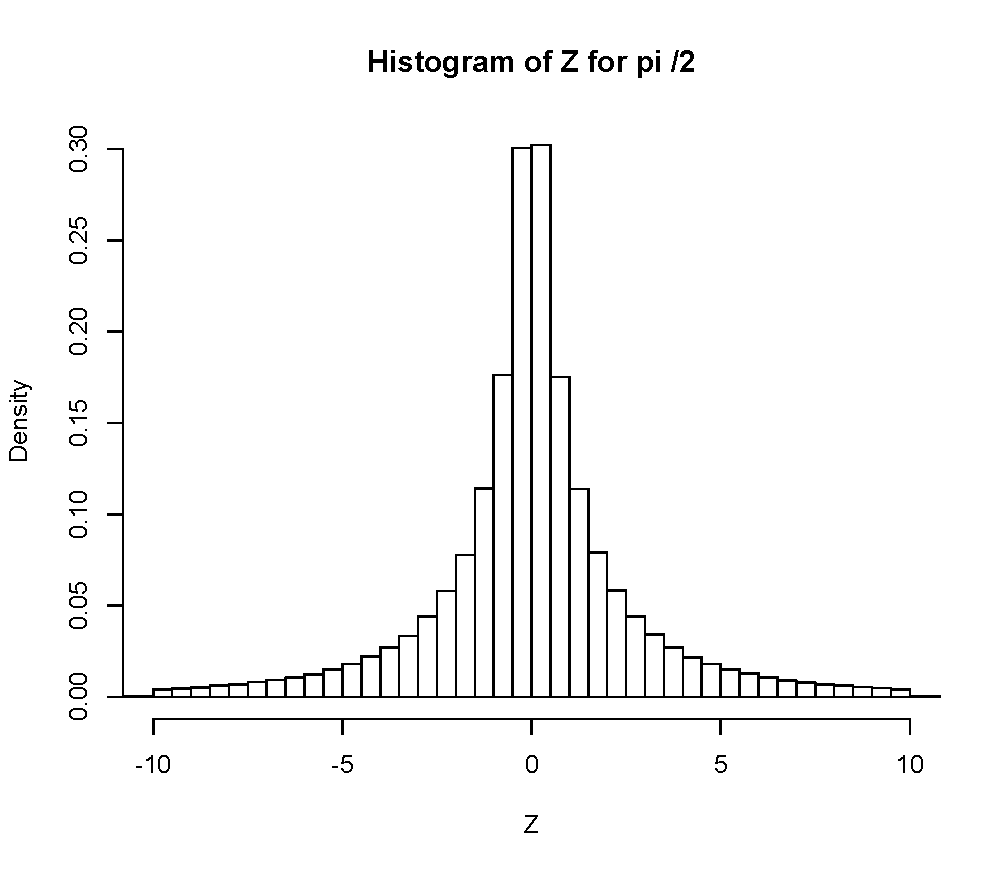
\includegraphics[width=0.8\textwidth]{pi2plot.pdf}
\caption[]{ 
 Distribution of zeta values at $\phi = \pi/2$.
  }
\vspace{1mm}
\label{pi2}
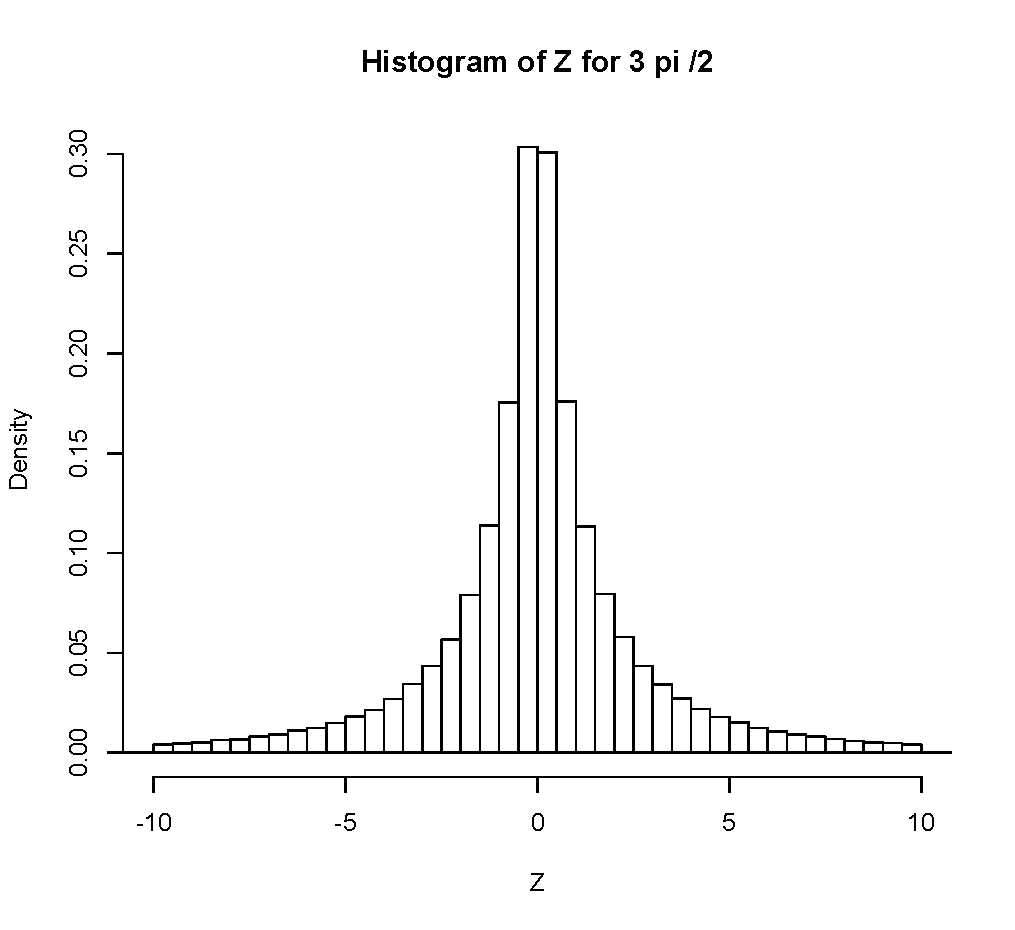
\includegraphics[width=0.8\textwidth]{3pi2plot.pdf}
\caption[]{ 
 Distribution of zeta values at $\phi = 3\pi/2$.
  }
\vspace{1mm}
\label{3pi2}
\end{figure*}

\subsection{\label{histograms}Histograms}
Ref.~\cite{Shanker 2018}  presented figures for the histograms at even and odd Gram points, which are the histograms for $\phi=0$ and $\phi=\pi$ respectively. Figs.~\ref{pi2} and \ref{3pi2} show 
the histograms for $\phi = \pi/2$ and $\phi = 3\pi/2$ respectively. Equation~\ref{eq:sym} predicts that the histograms have the same distribution. The figures validate this prediction to within the statistical precision.

Further, Equation~\ref{eq:antisym} predicts that the histograms are mirror images of each other.  For both relations to be valid, the distributions have to be symmetric. The figures also validate this fact. While  the histograms are symmetric, the distribution is not normal.  This can be seen from the kurtosis values in Table~\ref{tab:kurtosis4}  for $\phi = \pi/2$ and $\phi = 3\pi/2$.


\section{\label{sec4}Related work}
The value distribution of the Riemann zeta function has been well studied in the literature. We cannot cover all of this in the current work. We refer to Ivi\'c's monograph~\cite{Ivic 2013} for a comprehensive survey of  the field.
Selberg in unpublished work showed that at large $t$ $\log (\zeta(\frac{1}{2} + it))$ is approximately normally distributed with a standard deviation of order $\sqrt{log~log~t}$ (see Ref.~\cite{Hejhal}). He showed a 
similar result~\cite{Selberg 1989, Selberg 1991} for $\log (|Z(t)|)$. Laurincikas~\cite{Laurincikas}  used probabilistic number theory to prove various results about the distribution of the Riemann zeta function.

Regarding the value distribution at specific points along the Gram interval, we have already mentioned the work of Titchmarsh~\cite{Titchmarsh 1934} and Kalpokas and Steuding~\cite{kalpokas 2009} pertaining to the
mean value of the Riemann zeta function. Lester's~\cite{Lester 2013} Ph. D. thesis also considers the distribution of $\log (|\zeta(\frac{1}{2} + it)|)$  for specific points along the Gram interval. The anti-symmetry condition  Equation \ref{eq:antisym} and the symmetry condition  Equation \ref{eq:sym} of the current manuscript seem to be new. 

\section{\label{conclusions}Conclusions}

In this work we defined generalized Gram points on the critical axis, in analogy with Gram points. We used this definition to  formulate two new conjectures about the distribution of $Z(t)$ on the critical axis. We empirically observed  the mean value condition  Equation \ref{eq:mean}. This was stated and proved for Gram points by Ref.~\cite{Titchmarsh 1934}  and, as we discovered later,  for all $\phi$ in Ref.~\cite{kalpokas 2009}. 
Our two new results are the anti-symmetry condition  Equation \ref{eq:antisym} and the symmetry condition  Equation \ref{eq:sym}. Equation \ref{eq:antisym} is a generalization of Conjecture 1 in 
Ref.~\cite{Shanker 2018} to generalized Gram points.
The relations seem to hint at  profound new aspects of the behavior of the zeta function which have not yet been discovered. Theoretical study of the relations presented here needs to be done.

\section*{\label{appendix} Appendix}

\begin{table}
\centering \(\begin{array}{ccccccccccccc}
\hline
\phi & 0& \pi/6 &  \pi/3 &  \pi/2 & 2 \pi/3 & 5\pi/6 & \pi/ & 7\pi/6 & 4\pi/3 & 3\pi/2 & 5\pi/3 & 11\pi/6 \\
\hline
Standard& \\
deviation & 4.998& 5.002& 5.004& 5.004& 5.000& 4.996& 4.991& 4.987& 4.985& 4.986& 4.989& 4.993\\
\hline
\end{array}\)
\caption{Standard deviation for  $Z(t)$ when $\phi$ values are multiples of $\pi/6$.}
\label{tab:stddev6}
\end{table}

A more precise definition for the function $p_{phi}(y)$ is provided. We consider the interval along the critical axis specified by $(T_1, T_2)$. While empirical studies necessarily use large but finite  $T_1, T_2$, we are interested in the limit 
$T_1 \rightarrow \infty, T_2 \rightarrow \infty,  T_2-T_1 \rightarrow \infty,$ however
\begin{equation}
T_2 - T_1  \ll T_1. 
\label{eq:interval}
\end{equation}
Because of Equation \ref{eq:interval}, we can consider  $\ln (t)$  to be effectively constant over  the interval. A probability space $W$ is defined by a sample space of elementary events $\Omega$, a $\sigma$ algebra of all considered events $\mathcal{F}$, and a probability measure $P$. Our space of elementary events $\Omega$ is the set of all generalized Gram points with value phi in the interval. This is easily seen to be a discrete space. If we denote $\theta (T_1) = 2k_1\pi + \phi$, $\theta (T_2) = 2k_2\pi + \phi$, then we can index the set of generalized Gram points in the interval by the integer  $k$, where $k$ lies in the interval $(k_1, k_2)$. Since the mean spacing $\delta$ of the zeros at height $t$ is $\delta = 2\pi(\ln (t/2\pi))^{-1}$, the cardinality of this set is $(T_2 - T_1)*(\ln (T_1/2\pi))/(2\pi)$. Since we are dealing with a discrete space, we follow standard practice and choose $\mathcal{F}$,  the  $\sigma$ algebra, to be the collection of all subsets of $\Omega$ . Finally, the random variable whose probability distribution we wish to study is the value of $Z(t)$ at the generalized Gram point $t$.

It is not known whether the limiting probability distribution exists for $Z(t)$ at generalized Gram points. However, we can get some insight from the studies of Kalpokas and Steuding \cite{kalpokas 2009}. They show that for $\phi_1$ in the range $[0, \pi)$ 
\begin{equation}
\sum_{0 < t < T, \zeta(\frac{1}{2}+it) \in e^{i\phi_1}\mathbb{R}} \zeta(\frac{1}{2}+it) = (2e^{i\phi_1}\cos(\phi_1))\frac{T}{2\pi}\ln (\frac{T}{2\pi}) + O_\epsilon(T^{(\frac{1}{2}+\epsilon}).
\label{eq:kalpokas1}
\end{equation}
From Equation~\ref{eq:kalpokas1} and the cardinality of our sample space, it follows that a finite mean can be defined for the value distribution in our sample space. This gives support to the existence of a limiting distribution. We now consider the possibility of defining higher order moments for the value distribution. Kalpokas and Steuding  also show that
\begin{equation}
\sum_{0 < t < T, \zeta(\frac{1}{2}+it) \in e^{i\phi_1}\mathbb{R}} |\zeta(\frac{1}{2}+it)|^2 = \frac{T}{2\pi}(\ln (\frac{T}{2\pi}))^2 + (2\gamma+2\cos(2\phi_1))\frac{T}{2\pi}\ln (\frac{T}{2\pi}) + \frac{T}{2\pi} + O_\epsilon(T^{(\frac{1}{2}+\epsilon}),
\label{eq:kalpokas2}
\end{equation}
where $\gamma$ is Euler's constant. From Equation~\ref{eq:kalpokas2} and the cardinality of our sample space it seems that higher order moments of the value distribution diverge logarithmically. There is a lot of cancellation between positive and negative values of $Z(T)$ for odd moments, so odd moments will  behave better than even moments. It seems likely that a limiting value distribution exists, it has a finite well-defined mean, and higher moments diverge logarithmically. Distributions which do not have all moments defined are used in applications, for example, the Cauchy-Lorentz distribution~\cite{feller}. Equation~\ref{eq:kalpokas1} and \ref{eq:kalpokas2} predict that the standard deviation should be independent of $\phi$. This is verified in Table~\ref{tab:stddev6}.
 

\bibliographystyle{amsplain}
\begin{thebibliography}{10}


\bibitem{Shanker 2018} O. Shanker, 
``Good to Bad Gram Point Ratio For Riemann Zeta Function",
{\it Experimental Mathematics} {\bf doi:10.1080/10586458.2018.1492474}(2018)


\bibitem {Riemann(1858)} B. Riemann, ``\"{U}ber die Anzahl der Primzahlen uter
Einer Gegebenen Gr\"{o}be,'' {\it Montasb. der Berliner Akad.}, (1858),
671-680

\bibitem {Riemann 1892} B. Riemann, ``Gesammelte Werke'', Teubner, Leipzig, (1892)

\bibitem {Titchmarsh 1986} E. Titchmarsh, ``The Theory of the Riemann Zeta
Function,'' Oxford University Press, Second Edition, (1986)

\bibitem {Edwards(1974)} H. M. Edwards, ``Riemann's Zeta Function,''
Academic Press,  (1974)

\bibitem{Hardy 1918} G. H. Hardy and J. E. Littlewood,
``Contributions to the theory of the Riemann
zeta-function and the distribution of primes",
{\it Acta Math.} {\bf41}(1918), 119-196

\bibitem{Laurincikas} A. Laurincikas,
``Limit Theorems for the Riemann Zeta-Function",
Kluwer, Dordrecht, 1996

\bibitem{Gram 1903} J. P. Gram, 
``Sur les Zeros de la Fonction  $\zeta ( s )$  de Riemann",
{\it Acta Math.} {\bf27}(1903), 289-304

\bibitem{Titchmarsh 1934} E. C. Titchmarsh,
``On van der Corput's method and the zeta-function of Riemann (IV)",
{\it Quart. J. Math. Oxford Ser.} {\bf5}(1934), 98-105

\bibitem{kalpokas 2009} J. Kalpokas and J. Steuding,
``On the value-distribution of the Riemann zeta-function on the critical line", 
{\it Moscow Journal of Combinatorics and
Number Theory} {\bf1}(2011), 26-42

\bibitem{hiary 2010} G. A. Hiary,
``An amortized-complexity method to compute the Riemann zeta function", 
{\it Mathematics of Computation} {\bf80}(2011), 1785-1796

\bibitem{Odlyzko 1992}  A. Odlyzko,
``The $10^{20}$-th Zero of the Riemann Zeta
Function and 175 Million of its Neighbors", report,
\url{http://www.dtc.umn.edu/~odlyzko/unpublished/zeta.10to20.1992.pdf}, (1992)

\bibitem{hiary} G. A. Hiary,
``Fast methods to compute the Riemann zeta function",
{\it Annals of Mathematics} {\bf63}(1987), 891-946

\bibitem{gourdon} Xavier Gourdon,
``The $10^{13}$ first zeros of the Riemann Zeta function,
and zeros computation at very large height", report,
\url{http://numbers.computation.free.fr/Constants/Miscellaneous/zetazeros1e13-1e24.pdf}, (2004)

\bibitem {Ivic 2013} Aleksandar Ivi\'c, ``The Theory of Hardy's Z-Function,''
Cambridge University Press,  (2013)

\bibitem{Hejhal} D. A. Hejhal,
``On a result of Selberg concerning zeros of linear combinations
of L-functions", 
{\it Int. Math. Res. Not.} {\bf11}(2000), 551-577

\bibitem {Selberg 1989} A. Selberg, ``Selected Papers, Vol. I,''
Springer Verlag,  (1989)

\bibitem {Selberg 1991} A. Selberg, ``Selected Papers, Vol. II,''
Springer Verlag,  (1991)

\bibitem {Lester 2013} Stephen J. Lester, ``The Distribution of Values of the
Riemann Zeta-Function,''
Ph. D. dissertation, University of Rochester,  (2013)

\bibitem{feller} William feller,
``An Introduction to Probability Theory and Its Applications, Volume II (2 ed.)",
John Wiley and Sons, New York, 1971


\end{thebibliography} 

\end{document}


%-----------------------------------------------------------------------
% End of mcom-l-template.tex
%-----------------------------------------------------------------------
